
\begin{frame}{Modèles linéaires de correction}
    $$
    \mathsf{modeleCorrection} : \Delta \bm{p}_{\text{base}} \in \mathbb{R}^{3} 
    \longmapsto 
    \Delta \bm{p}_{\text{corrigé}} \in \mathbb{R}^{3}
    $$
    \vspace{1em}
    $$
    \only<1>{
        \begin{bmatrix}
            a_{0,0} & a_{0,1} & a_{0,2} & a_{0,3} \\
            a_{1,0} & a_{1,1} & a_{1,2} & a_{1,3} \\
            a_{2,0} & a_{2,1} & a_{2,2} & a_{2,3}
        \end{bmatrix}
    }
    \only<2>{
        \begin{bmatrix}
            0 & \textcolor[rgb]{1,0,0}{a_{0,1}} & 0 & 0 \\
            0 & 0 & \textcolor[rgb]{1,0,0}{a_{1,2}} & 0 \\
            0 & 0 & 0 & \textcolor[rgb]{1,0,0}{a_{2,3}}
        \end{bmatrix}
    }
    \only<3>{
        \begin{bmatrix}
            \textcolor[rgb]{1,0,0}{a_{0,0}} & \textcolor[rgb]{1,0,0}{a_{0,1}} & 0 & 0 \\
            \textcolor[rgb]{1,0,0}{a_{1,0}} & 0 & \textcolor[rgb]{1,0,0}{a_{1,2}} & 0 \\
            \textcolor[rgb]{1,0,0}{a_{2,0}} & 0 & 0 & \textcolor[rgb]{1,0,0}{a_{2,3}}
        \end{bmatrix}
    }
    \only<4>{
        \begin{bmatrix}
            \textcolor[rgb]{1,0,0}{a_{0,0}} & \textcolor[rgb]{1,0,0}{a_{0,1}} & \textcolor[rgb]{1,0,0}{a_{0,2}} & \textcolor[rgb]{1,0,0}{a_{0,3}} \\
            \textcolor[rgb]{1,0,0}{a_{1,0}} & \textcolor[rgb]{1,0,0}{a_{1,1}} & \textcolor[rgb]{1,0,0}{a_{1,2}} & \textcolor[rgb]{1,0,0}{a_{1,3}} \\
            \textcolor[rgb]{1,0,0}{a_{2,0}} & \textcolor[rgb]{1,0,0}{a_{2,1}} & \textcolor[rgb]{1,0,0}{a_{2,2}} & \textcolor[rgb]{1,0,0}{a_{2,3}}
        \end{bmatrix}
    }
    \begin{bmatrix}
        1 \\
        \Delta x_{\text{base}} \\   
        \Delta y_{\text{base}} \\   
        \Delta \theta_{\text{base}}
    \end{bmatrix}
    =
    \begin{bmatrix}
        \Delta x_{\text{corrigé}} \\   
        \Delta y_{\text{corrigé}} \\   
        \Delta \theta_{\text{corrigé}}
    \end{bmatrix}
    =
    \Delta \bm{p}_{\text{corrigé}}
    $$
    \vspace{1em}
    \begin{description}
        \item[Modèle proportionnel] :
            \alt<2>{\textcolor[rgb]{1,0,0}{$3$ paramètres}}{$3$ paramètres}
        \item[Modèle linéaire simple] : 
            \alt<3>{\textcolor[rgb]{1,0,0}{$6$ paramètres}}{$6$ paramètres}
        \item[Modèle linéaire complet] :
            \alt<4>{\textcolor[rgb]{1,0,0}{$12$ paramètres}}{$12$ paramètres}
    \end{description}
    \begin{itemize}
        \item Déplacement sur un cycle de marche (deux pas)
    \end{itemize}
\end{frame}

\begin{frame}{Expérimentation et identification}
    \begin{columns}
        \begin{column}{0.5\linewidth}
            Expérimentations :
            \begin{itemize}
                \item Pas de capteur externe
                \item Mesure manuelle de la pose finale
                \item Peu de séquences (20+5)
            \end{itemize}
            \vspace{1.0em}
            Identification par optimisation\\
            \vspace{1.0em}
            Fonction à minimiser :
            \begin{itemize}
                \item Distance entre poses estimées et observées
            \end{itemize}
        \end{column}
        \begin{column}{0.5\linewidth}
            \centering
            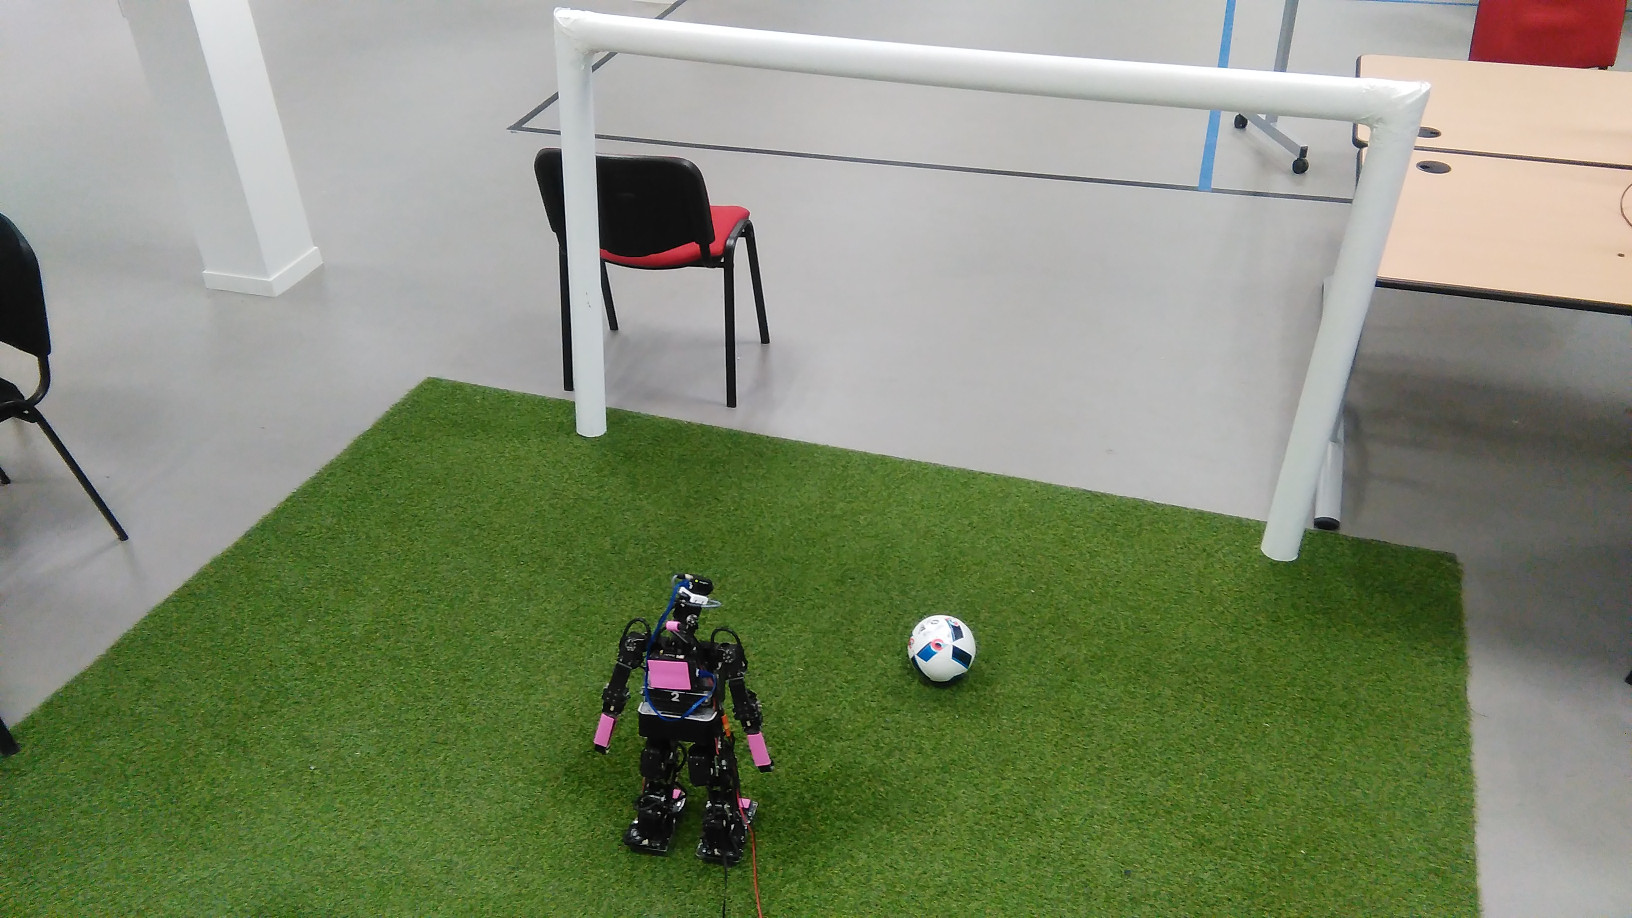
\includegraphics[width=1.0\linewidth]{../media/odometry_cmaes_setup.jpg}
            \vspace{1.0em}
            \small
        \end{column}
    \end{columns}
\end{frame}

\begin{frame}{Optimisation sans gradient}
    \begin{columns}
        \begin{column}{0.5\linewidth}
            \begin{block}{Optimisation sans gradient}
                (boite noire)
                \begin{itemize}
                    \item Fonction non linéaire, non convexe
                    \item Dérivées partielles non connues
                \end{itemize}
            \end{block}
            \vspace{1.0em}
            Covariance Matrix Adaptation Evolution Strategy (CMA-ES) :
            \begin{itemize}
                \item Algorithme génétique
                \item État de l'art \customtextcolor{(Hansen, 2009)}
                \item Implémentation C++ de référence
            \end{itemize}
        \end{column}
        \begin{column}{0.5\linewidth}
            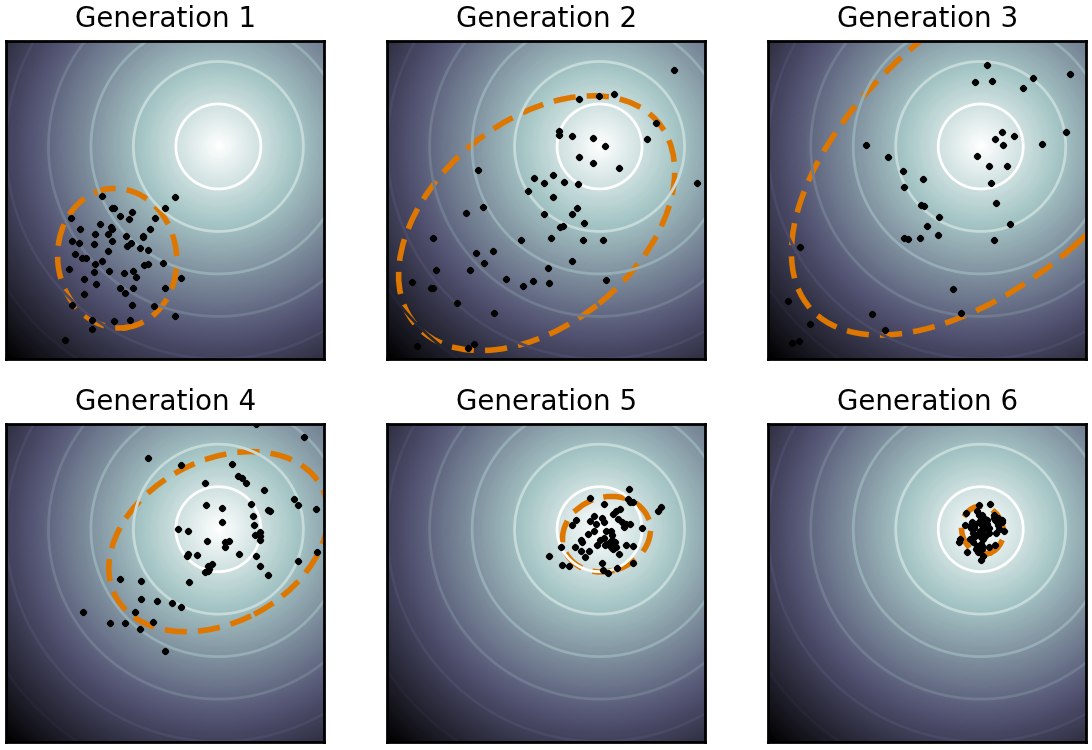
\includegraphics[width=1.0\linewidth]{../media/cmaes.png}\\
            \scriptsize
            (Source : wikipedia)
        \end{column}
    \end{columns}
\end{frame}

\begin{frame}{Résultats -- Comparaison des modèles}
    Après $\approx60$ pas, $20$~s\\
    \vspace{1.0em}
    \begin{columns}
        \begin{column}{0.5\linewidth}
            Odométrie prédictive :\\
            \vspace{1.0em}
            \centering
            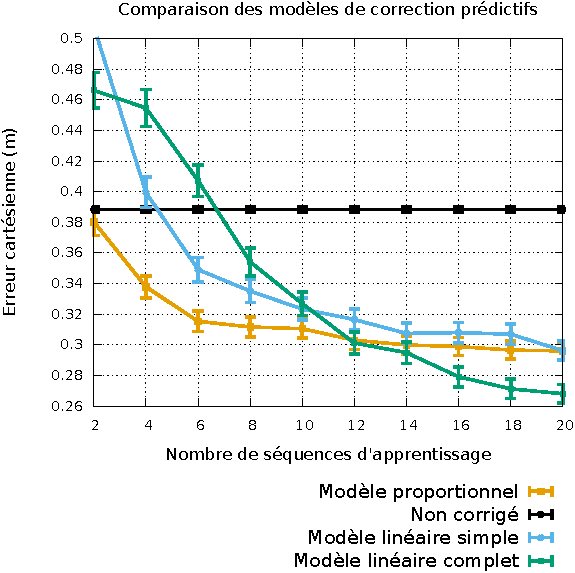
\includegraphics[type=pdf,ext=.pdf,read=.pdf,width=1.0\linewidth]{../plot/OdometryCMAES/convergenceOrders}
        \end{column}
        \begin{column}{0.5\linewidth}
            Odométrie proprioceptive :\\
            \vspace{1.0em}
            \centering
            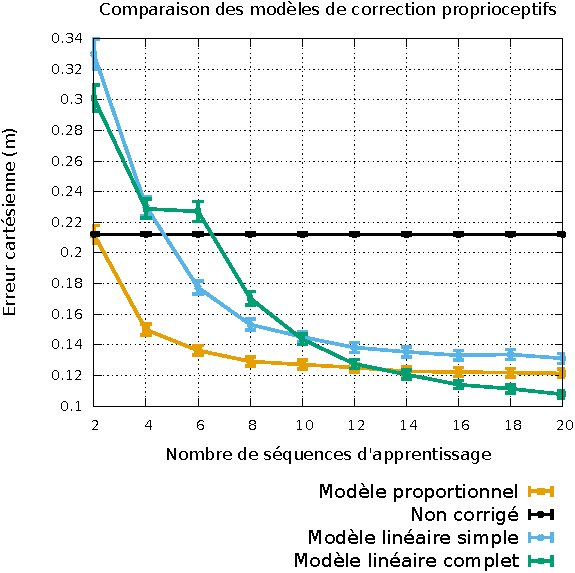
\includegraphics[type=pdf,ext=.pdf,read=.pdf,width=1.0\linewidth]{../plot/OdometryCMAES/convergenceReads}
        \end{column}
    \end{columns}
\end{frame}

\begin{frame}{Conclusion et applications}
    \begin{columns}
        \begin{column}{0.4\linewidth}
            Erreur cartésienne moyenne ($\approx60$ pas) :
            \begin{itemize}
                \item Prédiction :\\
                    $0.39$~m $\Rightarrow$ $\bm{0.27}$~m 
                \item Proprioception :\\
                    $0.21$~m $\Rightarrow$ $\bm{0.11}$~m 
            \end{itemize}
            \vspace{1.0em}
            Odométrie proprioceptive :\\
            $\Longrightarrow$ RoboCup 2016\\
            \vspace{1.0em}
            Odométrie prédictive :\\
            $\Longrightarrow$ Politique de contrôle du déplacement
        \end{column}
        \begin{column}{0.6\linewidth}
            \centering
            \movie[
                autostart,
                width=\linewidth, 
                height=0.56\linewidth,
                poster,
                loop
            ]{}{../video/cutICAPS2017_light.mp4}
        \end{column}
    \end{columns}
    \begin{block}{}
        \customtextcolor{
            \small
            \textit{An operational method toward efficient walk control policies for humanoid robots}}\\
        \scriptsize
        Ludovic Hofer, Quentin Rouxel\\
        ICAPS, 2017
    \end{block}
\end{frame}
